\chapter{Fundamental Concepts}
\label{cha:fundamentals}
\textbf{TODO: I -> We, no need to always say will, sometimes use passive to switch it up}
In this chapter I will lay out the fundamental concepts, which are necessary in order to understand the subsequent chapters.
First I will explain Stream Processing in \ref{sec:stream-processing}, afterwards the concept of the MAPE-K Loop will be presented and explained in subchapter \ref{sec:mape} 
followed by a brief explanation of self-adaptive systems in \ref{sec:self-adaptive} to conclude this chapter.

    \section{Stream Processing}
    \label{sec:stream-processing}
    In this section I will split the concept of Stream Processing into three further components.
    In \ref{sub:sps} I will then define Stream Processing Systems, explain how they work and give examplary fields of application.
    Afterwards in \ref{sub:dsms} I will then move onto the topic of Data Stream Management Systems and finally in \ref{sub:requirements} I will talk about
    some requirements that SPSs should meet.
    

        \subsection{Data Stream Management Systems}
        \label{sub:dsms}
        \ifbool{final}{}{\textbf{\color{green}THIS IS FINAL}
        
        }
        \textbf{NOT CLEAR ENOUGH, EXPLAIN LATENCY, CREATE DIAGRAM TO SHOW DIFFERENCE DBMS DSMS}
        A Data Stream Management is a system designed to manage continuous data streams.
        Similar to a DBMS a DSMS can also be queried using a streaming query language, however, queries installed on a DSMS are continuous 
        and will be executed as long as it is uninstalled.
        This leads to everchanging results, due to changing incoming data in contrast to querying a DBMS and receiving a static result.
        
        Another important difference is that the data being fed into the system is not saved like in DBMSs but instead only synopses, in 
        an attempt to summarize the data.
        
        Most notably the data being fed into a DSMS varies greatly from the data being inserted into a DBMS; while a DBMS receives a finite predetermined amount 
        of data, a DSMS could theoretically receive an infinite continuous stream.
        There are a few more functional differences, which Panigati, Schreiber and Zaniolo highlight, as shown in table 2.1.

        \begin{table}[h]
            \centering
            \label{tab:dbms-dsms}
            \begin{tabular}{|c|c|c|} \hline
                \textbf{Feature} & \textbf{DBMS} & \textbf{DSMS} \\ \hline
                Model & Persistent data & Transient Data \\ \hline
                Table & Set or bag of tuples & Infinite sequence of tuples \\ \hline
                Updates & All & Append only \\ \hline
                Queries & Transient & Persistent \\ \hline
                Query answers & Exact & Often approximate \\ \hline
                Query evaluation & Blocking and non-blocking & Non-blocking \\ \hline
                Operators & Fixed & Adaptive \\ \hline
                Data processing & Synchronous & Asynchronous \\ \hline
                Concurrency overhead  & High & Low \\ \hline
            \end{tabular}
            \captionbelow{Functional comparison of DBMS and DSMS\cite{Panigati2015}} 
        \end{table}

        \subsection{Stream Processing Systems}
        \label{sub:sps}
        \ifbool{final}{}{\textbf{\color{red}THIS IS NOT FINAL}
        
        }
        \textbf{TODO: Explain big data -> batch(latency low prio) and stream(latency high prio) }
        In this subsection I will explain what SPSs are, what their input looks like, what SPSs are able to do and give an example.
        In the end of this subsection I will also go over the challenges that SPSs face.

        % 1. Mehrere Generatoren generieren datenstroeme
        % -> Wie sieht ein Stream aus (infinite amount of tuples? see literature)
        % -> Was kann ein "Generator" sein? GPS Sensoren, EKG, EEG, .. (give few examples)
        Stream processing systems are fed continuous data streams, generated by data providers, for example GPS-sensors or EEG- and EKG-machines.
        Per definition of Panigati, Schreiber and Zaniolo\cite{Panigati2015} a data stream $S$ consists of a infinite, countable series of four-tuples $s := <\nu, t^{app }, t^{sys}, b_{id}>, s \in S$, where:

        \textbf{TODO: Replace this with a more general definition, e.g. from fundamentals of stream processing book}
        \begin{itemize}
        \item $\nu \in \mathfrak{R}$ is a relational tuple

        \item $t^{app} \in T$, with $T$ being the time domain, is a partially ordered application time
        
        \item $t^{sys} \in T$,  with $T$ being the time domain, is a totally ordered system time
        
        \item $b_{id} \in B$ is a batch id; batch $B$ is a finite subset of $S$ where all $b \in S$ have an identical $t^{app}$
        \end{itemize}

        % 2. Diese werden im SPS verarbeitet
        % -> Beispiel filtering        
        Each element \textit{s} then is processed by one or more operators, each doing their own independent operation, e.g. filtering as shown in figure \ref{fig:filter} \textbf{(somehow ref wrong?)}
        and then put out into the operator's outgoing stream.

        % -> Windows erklären (Tumbling, sliding) (grafiken zum Vergleich zeigen)
        \textbf{TODO: Implement some structure, not own sections but little headers maybe or new paragraphs or something}
        -> explain windows

        -> exanpe aggregation Tumbling

        -> example aggregation sliding

        -> elaborate Difference

        % -> Replication of operators zeigen
        In order to increase efficiency, an SPS can, if (computational) resources are available, create replicas of operators to introduce parallelity, as shown in figure \ref{fig:sps_parallel_normal} \textbf{Ref wrong?}. 
        Conversely, if there is little input, it may also reduce the amount of replicas in order to save or free up additional resources.

        
        % 3. SPS kann gequeried werden
        % -> Eventuell Beispiel geben
        
        % 4. SPS gibt Stream aus, welcher auf verschiedene Arten weiter verwaltet wird
        % -> Resultate können bspw. gespeichert werden, siehe graph
        % -> Outputstream kann auch weiter verarbeitet werden von anderen Systemen

        % 5. Challenges
        % -> e.g. Correctness 

        \begin{figure}[h]
        \label{fig:sps_parallel_normal}
        \centering
        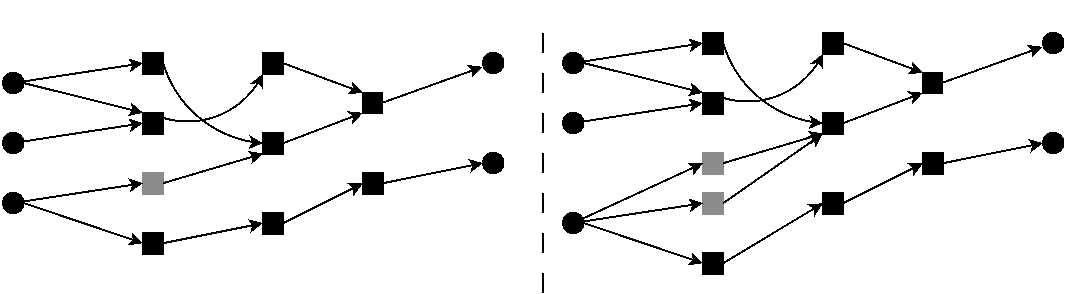
\includegraphics[width=1.0\textwidth]{Bilder/sps_parallel_normal.png}
        \caption{
                Left: An example for an SPS displayed as a directed acyclic graph. 
                Right: Same SPS with introduced parallelity in one operator, marked gray for visibility. 
                Circles are input/outputs, squares are operators, arrows are streams.
                TODO: EXPLAIN graph and sink, generator, processor!!
                }
        \end{figure}

        \begin{figure}
        \label{fig:stream-processing-system}
        \centering
        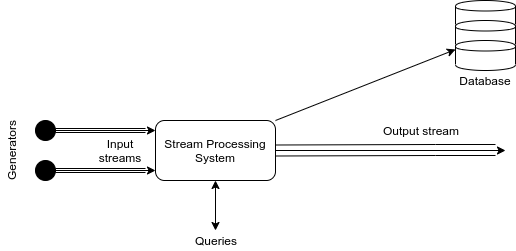
\includegraphics[width=1.0\textwidth]{Bilder/stream-processing-system.png}
        \caption{
                Overview of a basic Stream Processing System
                }
        \end{figure}  

        % Subsection Requirements for Stream Processing Systems
        % Should quickly go over the requirements and explain why they matter to us
        \subsection{Requirements for Stream Processing Systems}
        \label{sub:requirements}
        \ifbool{final}{}{\textbf{\color{red}THIS IS NOT FINAL}
        
        }

        Notes: What are the requirements, why do they matter to us (Elaborate on this)

        Due to the nature of the fields in which SPS are used, there are important requirements that SPS should meet in order to be viable, 
        which Stonebraker et al. point out in \cite{Stonebraker:2005:RRS:1107499.1107504}, of which the ones most important to us can be summarized as the following:
        
        % Enumeration of requirements for SPS + explanations why they matter to us
        \begin{enumerate}
        \label{enum:requirements}
            \item \textbf{Keep the Data Moving:} 
                In order to minimize latency, data must not be stored, as these are costly operations.
            \item \textbf{Handle Stream Imperfections:} 
                Expecting only perfect data is utopian, so one must prepare the system with built-in mechanisms for data that might be missing or out-of-order.
            \item \textbf{Integrate Stored and Streaming Data:} 
                For an SPS to be able to perform comparisons between "predecessor" data and current data, operators must keep an efficiently manageable state.
            \item \textbf{Guarantee Data Safety and Availability:} 
                Recovering from a failure is detrimental for real-time data processing, so a system must be in place to guarantee the highest availability possible.
            \item \textbf{Process and Respond Instantaneously:} 
                Systems must be highly optimized in order to provide (near) real-time responses.
            \item \textbf{Partition and Scale Applications Automatically:} 
                Systems must be able to be split across multiple machines and threads.
                The system must also be able to automatically scale and distribute the load across the machines.

        \end{enumerate}

    \section{MAPE-K Loop}
    \label{sec:mape}
    \ifbool{final}{}{\textbf{\color{green}THIS IS FINAL (Maybe add something underneath enum if not sufficient)}
    
    }{}
    % Explain the MAPE-K Loop as it is a valuable basis/reference architecture for many different approaches in adaptive systems
    % Rough explanation of what it is, where it is used
    % explain different "stages" (m, a, p, e)
    % Explain -K extension
    The MAPE-K Loop was introduced by IBM \cite{Kephart:2003:VAC:642194.642200} and refers to a proposed solution for self-adaptive or autonomic systems.
    This model has since become the basis or reference architectural pattern for many self adaptive systems, which I will show in the third chapter.
    The acronym MAPE-K refers to the components that make up the model:
    \textbf{TODO: Add a diagram, make this a subsection of self-adaptive systems}
    \begin{enumerate}
    \label{enum:mape}
        \item \textbf{M}onitor: 
            The \textit{Monitor} component gathers data about the system and its environment, aggregates and filters it.
        \item \textbf{A}nalyze: 
            The \textit{Analyze} component analyzes the previously gathered data and determines whether or not an adaptation should be performed.
            The decision is made based on performance or cost gain and should include the adaptation cost as well.
            This component's analysis is influenced by the \textit{Knowledge} base.
        \item \textbf{P}lan: 
            If the choice to adapt the system has been made, the \textit{Plan} component then decides how to reconfigure the system.
            Once the decision has been made, the information is then forwarded to the \textit{Execute} component.
        \item \textbf{E}xecute: 
            Given the \textit{Plan} component's decision, the \textit{Execute} component then executes said plan and the loop 
            returns to the initial monitoring state.
        \item \textbf{K}nowledge: 
            Represents the knowledge base, which is shared between the other components.
            This base is created by the \textit{Monitor} component and contains information in the form of metrics, policies, symptoms and logs.
    \end{enumerate}

    
    \section{Self-Adaptive Systems}
    \label{sec:self-adaptive}
    \ifbool{final}{}{\textbf{\color{green}THIS IS FINAL?}
    
    }{}
    \textbf{Needs more; e.g why self-adaptive(already mentioned in intro), Software engineering perspective on self adaptivity, challenges}
    % Definition of self-adaptive systems
    % Architecture often based on mape in different patterns
    % applied in xx industries
    Cheng et al. define self-adaptive systems as
    \begin{quotation}
        ``[...] systems that are able to adjust their behaviour in response to their perception of the environment and the
        system itself [...]``\cite[p.1]{Cheng:2009:SES:1573856.1573858}.
    \end{quotation}
    
    Self-adaptive systems are oftentimes based on the \nameref{sec:mape} [p.\pageref{sec:mape}] pattern.
    Adaptive Systems have a wide variety of possible application areas: adaptable user interfaces, autonomic computing, multi-agent systems \cite{Cheng:2009:SES:1573856.1573858}, 
    biologically inspired computing, robotics \cite{10.1007/978-3-319-59480-4_44}, streaming applications and a lot more.

    An examplary application would be a scenario, in which population and food capacities are given and evolving over time, due to births, deaths, changes in demographics 
    and changes in weather and harvest respectively. A system would have to adapt to these changes in its environment in order to ration the food properly.


\chapter{Approaches for Self-Adaptive Architectures in Stream Processing}
\label{cha:approaches}
\textbf{TODO: How does it work? FOCUS ON ARCHITECTURE IN THIS CHAPTER!!}
Explain that this chapter showcases a few select strategies, which are then elaborated on further in the subchapters
Question: Even more approaches? e.g. Master-Slave pattern or Coordinated Control pattern (Both MAPE based)?
\textbf{Add and explain a few more MAPE Based architectures}

    \section{Dhalion}
    \label{sec:dhalion}
    Quick Introduction to Dhalion, this chapter will deal with the Dhalion paper.
    NOTE: Explain what Dhalion is, where its used

        \subsection{An Outline of Heron}
        \label{sub:heron-outline}
        Small outline of Heron, as Dhalion is built on top of Twitter's Heron.

        \subsection{Dhalion's Architecture}
        \label{sec:dhalion-architecture}
        \textbf{TODO: Diagram, explain it here}
        Explanation of Dhalion's Architecture \textbf{KERNPUNKT DER SECTION DHALION}

        \subsection{Discussion of Dhalion}
        \label{sec:dhalion-discussion}
        Discuss the approach and compare it to the reference architecture (Mape?)
        \textbf{TODO: Maybe discuss how they evaluate, look at metrics relevant to architecture}

    \section{Decentralized Self-Adaptation}
    \label{sec:hierarchical}
    \textbf{TODO: Incorporate same structure as above}
    NOTE: In this section I will explain the hierarchical control architecture as decribed by Cardellini..

        \subsection{Elastic and Distributed DSP Framework}
        \label{sec:edf}
        \textbf{TODO: Possibly change title of this, add diagram, explain thoroughly (decentralized etc.), extract their design patterns}
        Explanation of the EDF, their architecture for elastic DSP apps \textbf{KERNPUNKT DER SECTION}

        \subsection{Discussion of EDF}
        \label{sec:discussion-edf}

    \section{Some Other Architecture}
    \label{sec:soa}
    NOTE: In this chapter I will explain another architecture/approach to self-adaption, yet to be researched


    \section{Some Other Architecture2}
    \label{sec:soa2}
    NOTE: In this chapter I will explain another architecture/approach to self-adaption, yet to be researched


    \section{Title??}
    \textbf{TODO: Discuss among all of them, critical thinking..}

    \textbf{TODO: If enough material compare the architecture relevant metrics of the approaches}